\chapter{Lecciones de la vida}

Gracias al paquete\td{esta es una nota en línea, con la macro \texttt{\textbackslash td\{\}}} \texttt{inputenc} (cargado como \texttt{\textbackslash usepackage[utf8]{inputenc}}), podemos escribir en español sin ningún problema. Ejemplos: tíĺdéś. \todo{Esta es una nota de cosas pendientes, con el comando \texttt{\textbackslash todo\{text\}}.}
%привет



\section{Referidas a los alimentos}\label{sec:cap1:alimentos}

\subsection{Burbujas quemadas de las galletas de agua}

\subsubsection{Por qué son malas}

\subsubsection{Cómo sacarlas}

\subsubsection{Análisis de mercado}

\minisec{Traviata} % Minisec es de las clases de Koma-Script

Las galletas \nombre{Traviata} son de las preferidas por el mercado, especialmente para sopar en té negro dulce. Sin embargo, tal como se observa en la \cref{fig:traviatas_ej1}\footnote{Normalmente, \texttt{cref} es la opción preferible para citar, ya que automáticamente añade el tipo de referencia, y es mejor que \texttt{autoref} del paquete \texttt{hyperref}. Sin embargo, puede ser útil usar el tradicional \texttt{ref} en otros casos.}, a veces tienen muchas burbujas quemadas. El nivel de quemazón no es estable, y el consumidor afortunado puede encontrar un paquete de galletas sin burbujas quemadas. Son las menos; normalmente uno encontrará unas como las que se ven en la figura\footnote{En español los nombres de elementos comunes como \enquote{figura}, \enquote{sección}, \enquote{tabla}, se escriben en con minúscula inicial. Escribirlos con mayúscula es un anglicismo, según la \nombre{Fundéu BBVA} via mail privado.\label{notamayusculas}} \ref{fig:traviatas_ej2}. Esto es con \texttt{autoref}: \autoref{fig:traviatas_ej1}, \autoref{fig:traviatas_ej2}, y no esta bueno por lo dicho en la \cref{notamayusculas}.


En este párrafo uso el paquete \programa{cleverref} para referenciar. Por ejemplo, hago referencia a la \cref{fig:traviatas}, o a la \cref{sec:cap1:alimentos}, o a las \cref{fig:traviatas_ej1,fig:traviatas_ej2}.

\texttt{Cleveref} también me permite referenciar números de página. Por ejemplo, puedo pedir que lean la página \pageref{sec:cap1:alimentos}.

También puedo insertar los nombres de las referencias: lean la \cref{sec:cap1:alimentos}, \nameref{sec:cap1:alimentos}.




% Ejemplo de dos imágenes en línea
\begin{figure}
    \centering
    %
    \begin{subfigure}[b]{0.4\linewidth}
        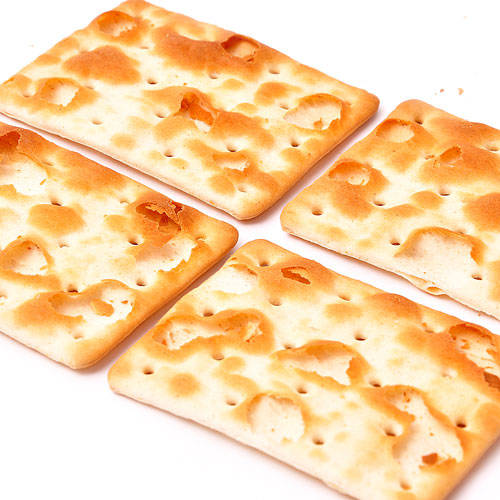
\includegraphics[width=1\linewidth]{traviatas}
        \caption[Traviatas]{Ejemplo 1.}
        \label{fig:traviatas_ej1}    
    \end{subfigure}
    %
    \hfill % llena el espacio entre figuras, para ocupar todo el ancho
    %
    \begin{subfigure}[b]{0.4\linewidth}
        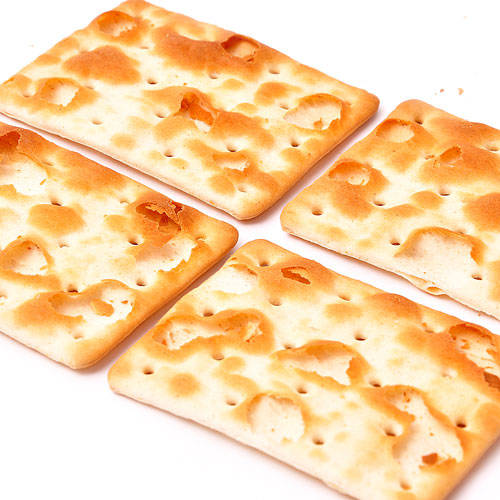
\includegraphics[width=1\linewidth]{traviatas}
        \caption[Traviatas]{Ejemplo 2.}
        \label{fig:traviatas_ej2}    
    \end{subfigure}
    %
    \caption[Traviatas]{Estas son galletas \nombre{Traviata} con burbujas quemadas.}
    \label{fig:traviatas}    
\end{figure}




% Ejemplo de 3 imágenes en línea
\begin{figure}
    \centering
    %
    \begin{subfigure}[b]{0.3\linewidth}
        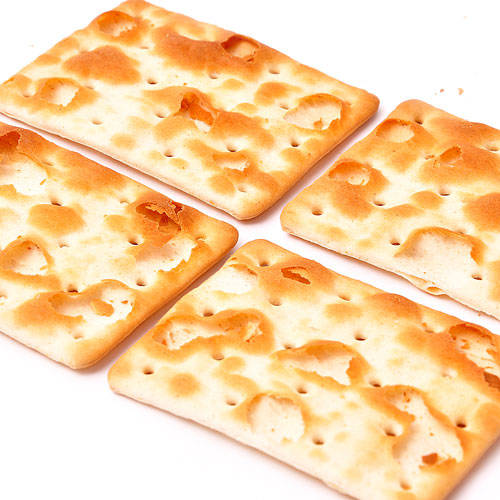
\includegraphics[width=1\linewidth]{traviatas}
        \caption[Traviatas]{Ejemplo 1.}  
    \end{subfigure}
    %
    \hfill % llena el espacio entre figuras, para ocupar todo el ancho
    %
    \begin{subfigure}[b]{0.3\linewidth}
        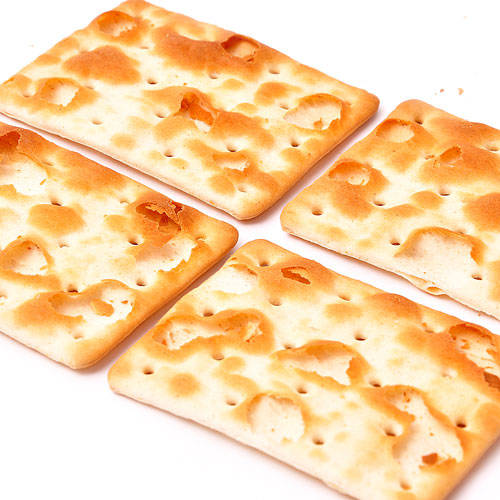
\includegraphics[width=1\linewidth]{traviatas}
        \caption[Traviatas]{Ejemplo 2.} 
    \end{subfigure}
    %
    \hfill % llena el espacio entre figuras, para ocupar todo el ancho
    %
    \begin{subfigure}[b]{0.3\linewidth}
        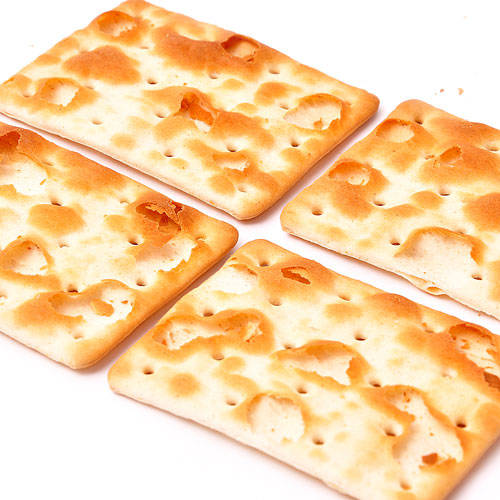
\includegraphics[width=1\linewidth]{traviatas}
        \caption[Traviatas]{Ejemplo 3.} 
    \end{subfigure}
    %
    \caption[Traviatas]{Estas son galletas \nombre{Traviata} con burbujas quemadas.}
    \label{fig:3traviatas}    
\end{figure}




% Ejemplo de cuatro subimágenes en dos filas
\begin{figure}
    \centering
    %
    \begin{subfigure}[b]{0.2\linewidth}
        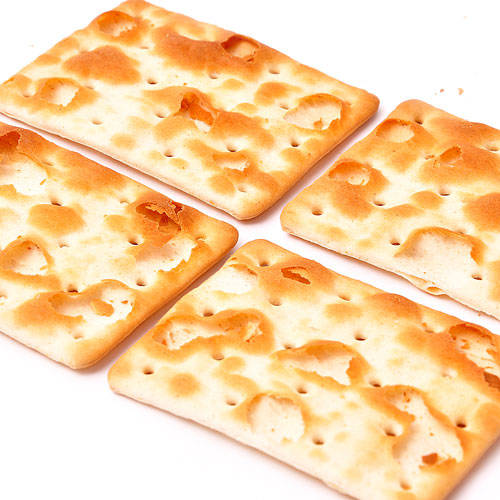
\includegraphics[width=1\linewidth]{traviatas}
        \caption[Traviatas]{Ejemplo 1.}  
    \end{subfigure}
    %
%    \hfill % llena el espacio entre figuras, para ocupar todo el ancho
    %
    \begin{subfigure}[b]{0.2\linewidth}
        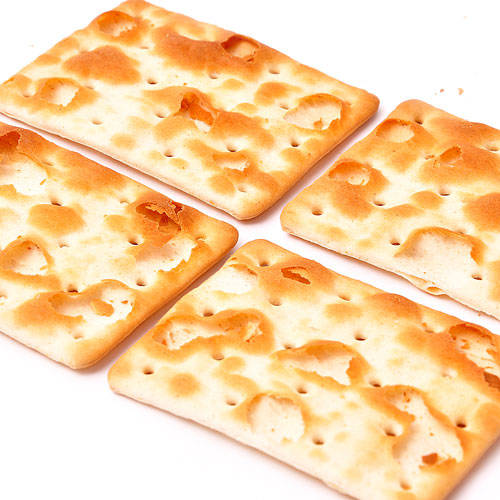
\includegraphics[width=1\linewidth]{traviatas}
        \caption[Traviatas]{Ejemplo 2.} 
    \end{subfigure}
    %
    \\ % salto de línea
    %
    \begin{subfigure}[b]{0.2\linewidth}
        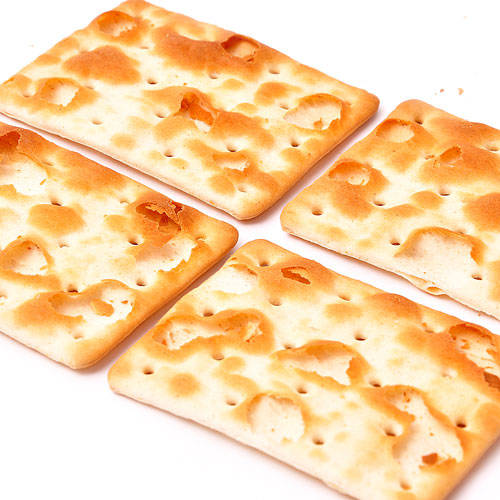
\includegraphics[width=1\linewidth]{traviatas}
        \caption[Traviatas]{Ejemplo 3.}  
    \end{subfigure}
    %
%    \hfill % llena el espacio entre figuras, para ocupar todo el ancho
    %
    \begin{subfigure}[b]{0.2\linewidth}
        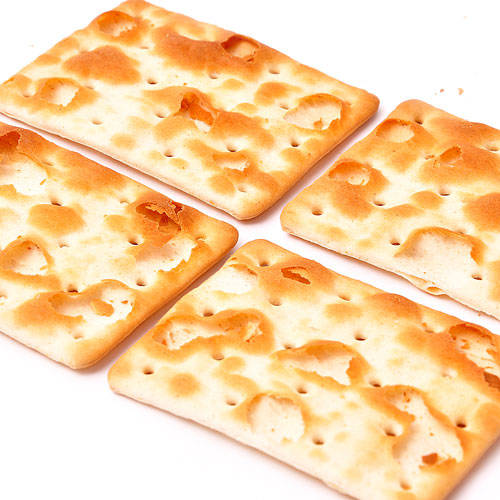
\includegraphics[width=1\linewidth]{traviatas}
        \caption[Traviatas]{Ejemplo 4.} 
    \end{subfigure}
    %
    \caption[Traviatas]{Estas son galletas \nombre{Traviata} con burbujas quemadas.}
    \label{fig:4traviatas}    
\end{figure}



% Ejemplo de cuatro subimágenes en dos filas, pero con más espacio horizontal y vertical
\begin{figure}
    \centering
    %
    \begin{subfigure}[b]{0.2\linewidth}
        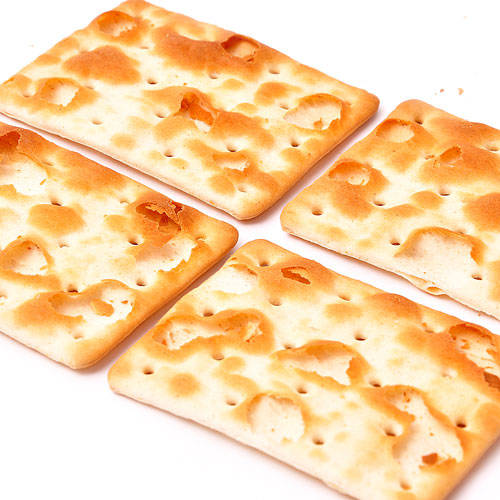
\includegraphics[width=1\linewidth]{traviatas}
        \caption[Traviatas]{Ejemplo 1.}  
    \end{subfigure}
    %
    \hspace{0.1\linewidth} % espacio horizontal
    %
    \begin{subfigure}[b]{0.2\linewidth}
        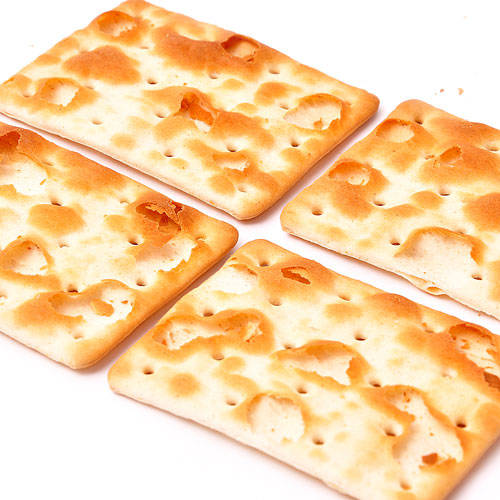
\includegraphics[width=1\linewidth]{traviatas}
        \caption[Traviatas]{Ejemplo 2.} 
    \end{subfigure}
    %
    \\ % salto de línea
    \vspace{0.1\linewidth} % espacio vertical
    %
    \begin{subfigure}[b]{0.2\linewidth}
        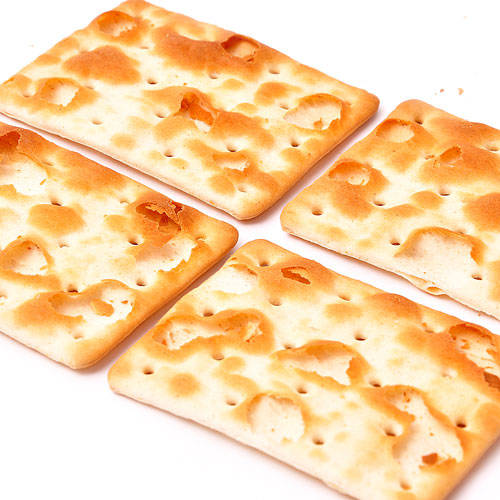
\includegraphics[width=1\linewidth]{traviatas}
        \caption[Traviatas]{Ejemplo 3.}  
    \end{subfigure}
    %
    \hspace{1em} % espacio horizontal
    %
    \begin{subfigure}[b]{0.2\linewidth}
        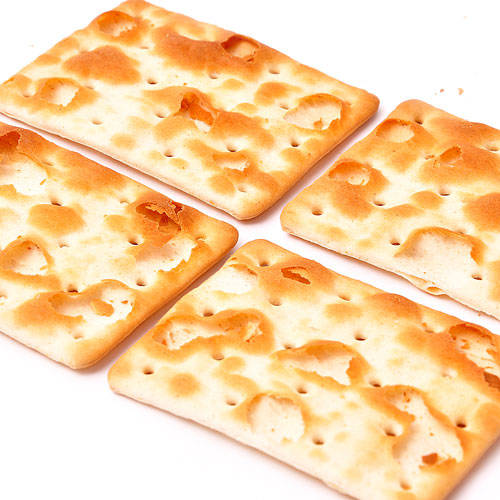
\includegraphics[width=1\linewidth]{traviatas}
        \caption[Traviatas]{Ejemplo 4.} 
    \end{subfigure}
    %
    \caption[Traviatas]{Estas son galletas \nombre{Traviata} con burbujas quemadas.}
    \label{fig:4traviatas_otras}    
\end{figure}




\minisec{Criollitas}

Este es un párrafo de las \nombre{Criollitas}.


\minisec{Mediatarde}

Este es un párrafo de las \nombre{Mediatarde}.


\paragraph{Hogareñas} Este párrafo referido a las galletas \nombre{Hogareñas} está hecho con \texttt{\textbackslash paragraph\{\}} en lugar de \texttt{\textbackslash minisec\{\}}. Es otra opción de encabezado menor. Probablemente sea mejor que \texttt{minisec}, para mantener uniformidad.

Y la \cref{tabla:tabladeejemplo} es una tabla de ejemplo.

\begin{table}[hbt]
    \centering
    \caption[Cultivos de almendra en Argentina en 2015]{cultivos de almendra en Argentina en 2015.~\autocite{iannamico:cultivo}}
    \label{tabla:tabladeejemplo}
    \begin{tabular}{@{}lr@{}}
        \toprule
        Provincia           & Superficie cultivada {[}Ha{]} \\ \cmidrule{1-2} % o \midrule
        Mendoza             & 2580                          \\
        San Juan            & 572                           \\
        La Rioja            & 498                           \\
        Salta               & 189                           \\
        Río Negro y Neuquén & 170                           \\
        Otras               & 200                           \\
        Total               & 4209                          \\ \bottomrule
    \end{tabular}
\end{table}


Acá un poco del uso de \nombre{SIUnitx} para el formato de números y unidades. \SI{30}{\kg},  \SI{80}{\percent}, \num{2015}, \num{40000}, \SI{800x600}{\pixel}, \num{640x480}, \ang{45}, \SIrange{10}{20}{\kilogram}, \SIlist{1;2;3}{\metre} , \SIrange{1}{10}{\degreeCelsius}, \SI{12.3(2)}{\kilogram}. También funciona en modo matemático:
$ \SI{15000}{\micro\gram} $




\pagebreak

Agrego por último unas ecuaciones de ejemplo. Se determinan a continuación la media circular y la desviación estándar circular, que se usaron como descriptores de color.~\autocite{estcirc}

% PREGUNTAR SI ECUACIÓN CON NÚMEROS. IMPLICARÍA QUE LAS DE LOS CLASIFICADORES TAMBIÉN TENGAN...
Sea un conjunto de $ n $ ángulos $ a_1, a_2, \dots, a_n $. Estos pueden interpretarse como $ n $ vectores $ \bm{v} $ de magnitud $ 1 $ y ángulos $ a_1, a_2, \dots, a_n $ respectivamente:
%
\begin{equation} \bm{v_n} = 1 e^{j a_n} \end{equation}
%
Si se convierten a coordenadas cartesianas, se tiene:
%
\begin{equation} \bm{v_n} = \cos(a_n) + j \sin(a_n) \end{equation}
%
Sumando los $ n $ vectores obtenemos el vector resultante $ \bm{a} $:
%
\begin{equation} \bm{a} = \sum_{1}^{n} \bm{v_n} = R e^{j \rho} \end{equation}
%
La \textbf{media circular} (o \textbf{ángulo medio} en este caso) es el ángulo $ \rho $ descripto por este vector resultante $ \bm{a} $.
%
La longitud media de los vectores $ \bm{v_n} $ se define como:
%
\begin{equation} \bar{R} = \frac{R}{n} \end{equation}
%
Y la \textbf{desviación estándar circular} como:
%
\begin{equation} S = \sqrt{\ln\left(\frac{1}{\bar{R}^2}\right)} = \sqrt{-2 \ln \left( \bar{R}^2 \right) } \end{equation}


\paragraph{Un poco de código}

A continuación, un poco de código de \nombre{Matlab}, usando el paquete \programa{listings}.\footnote{Ver también el paquete \programa{minted}, se ve muy interesante.}


\lstinputlisting[style=Matlab-editor, basicstyle=\small, caption = {Cálculo del vector de covarianza de dos señales.}]{codigo/matlab.m}



Y un poco más de código, pero esta vez en C++:
% NOTA: Puedo incluirlo así porque no tiene caracteres no ASCII. 
% Lo más fácil, para evitar problemas extraños, es no incluir el código dentro
% del archivo .tex, sino importarlo desde archivos externos. Esto implica no
% usar el entorno 'lstlisting' sino usar el comando
% \lstinputlisting[opciones]{archivo}
\begin{lstlisting}[language=c++, caption = {Swap values (https://cpppatterns.com/patterns/swap-values.html)}, title=Swap values]
#include <utility>
#include <string>

int main() {

  std::string s1 = "Hello";
  std::string s2 = "World";
  using std::swap;
  swap(s1, s2);
  
}
\end{lstlisting}